\documentclass{article}

% NeurIPS 2026 main conference format: 140 cm (W) x 90 cm (H), landscape.
\usepackage[paperwidth=140cm, paperheight=90cm, margin=0mm]{geometry}

\usepackage[T1]{fontenc}
\usepackage{lmodern}
\usepackage[default]{sourcesanspro}
\usepackage{scrextend}
\changefontsizes[34pt]{27pt}

\usepackage{amsmath}
\usepackage{amssymb}
\usepackage{xcolor}
\usepackage{graphicx}
\usepackage{booktabs}
\usepackage{colortbl}
\usepackage{makecell}
\usepackage{pifont}
\usepackage{listings}
\usepackage{qrcode}
\usepackage{hyperref}
\usepackage[poster]{tcolorbox}
\usepackage{symbols}

\definecolor{themecolor}{RGB}{26,129,235} % TorchJD logo blue
\definecolor{darktext}{RGB}{35,35,45}
\definecolor{pagebg}{RGB}{246,246,248}
\colorlet{tablerow}{themecolor!8}

\hypersetup{colorlinks, allcolors=themecolor}
\color{darktext}

\newcommand{\cmark}{{\color{green!60!black}\ding{51}}}
\newcommand{\xmark}{{\color{red!75!black}\ding{55}}}
\newcommand{\hl}[1]{{\color{themecolor}\textbf{#1}}}

\lstdefinestyle{pythonstyle}{
    language=Python,
    basicstyle=\ttfamily\small,
    keywordstyle=\color{blue}\bfseries,
    commentstyle=\color{green!50!black},
    stringstyle=\color{red},
    showstringspaces=false,
    columns=fullflexible,
    keepspaces=true,
}

% Highlighted statement inside a box (definitions, theorem).
\newtcolorbox{keybox}[1][]{
    enhanced, colback=themecolor!6, colframe=themecolor!6, boxrule=0pt, arc=3mm,
    left=8mm, right=8mm, top=4mm, bottom=4mm, borderline west={3mm}{0pt}{themecolor}, #1
}

\pagecolor{pagebg}

\begin{document}
\begin{tcbposter}[
    coverage={spread, interior style={fill=pagebg}},
    poster={columns=4, rows=40, colspacing=18mm, rowspacing=10mm, spacing=20mm, showframe=false},
    boxes={
        enhanced, colback=white, colframe=white, boxrule=0pt, arc=4mm,
        left=12mm, right=12mm, top=6mm, bottom=8mm,
        colbacktitle=white, coltitle=themecolor, fonttitle=\bfseries\huge, halign title=flush left,
        titlerule=1.5mm, titlerule style={themecolor}, toptitle=6mm, bottomtitle=3mm,
        left skip=0mm, right skip=0mm,
        before upper={\setlength{\parskip}{0.6em}},
        drop fuzzy shadow=black!25,
    },
]

%%%%%%%%%%%%%%%%%%%%%%%%%%%%%%%%%%%%%%%%%%%%%%%%%%%%%%%%%%%%%%%%%%%%%%%%%%%%%%%%%%%%%%%%%%%%%%%%%%%%%%%%%%%%%%%%%%%%%%%%%%
% Header
\posterbox[colback=themecolor, colframe=themecolor, colupper=white, halign=center, valign=center, top=14mm, bottom=14mm,
           height=12.5cm]{name=header, column=1, span=4, below=top}{
    \begin{minipage}[c]{0.09\linewidth}
        \centering
        \fcolorbox{white}{white}{\color{black}\qrcode[height=8cm, nolink]{https://arxiv.org/abs/2406.16232}}\\[4mm]
        {\large Paper}
    \end{minipage}%
    \hfill
    \begin{minipage}[c]{0.13\linewidth}
        \centering
        
\includegraphics[width=\linewidth]{images/logos/simplexlab_white.pdf}
    \end{minipage}%
    \hfill
    \begin{minipage}[c]{0.54\linewidth}
        \centering
        {\fontsize{92}{110}\selectfont\bfseries Jacobian Descent for Multi-Objective Optimization\par}
        \vspace{14mm}
        {\Huge Pierre Quinton$^\ast$ {\Large(LTHI, EPFL)} \hspace{2.5cm} Val\'erian Rey$^\ast$ {\Large(SimplexLab)}\par}
        \vspace{4mm}
        {\large $^\ast$Equal contribution\par}
    \end{minipage}%
    \hfill
    \begin{minipage}[c]{0.13\linewidth}
        \centering
        
\includegraphics[width=\linewidth]{images/logos/torchjd_white.png}
    \end{minipage}%
    \hfill
    \begin{minipage}[c]{0.09\linewidth}
        \centering
        \fcolorbox{white}{white}{\color{black}\qrcode[height=8cm, nolink]{https://github.com/SimplexLab/TorchJD}}\\[4mm]
        {\large Code}
    \end{minipage}
}

% Take-home message
\posterbox[colback=themecolor!8, colframe=themecolor!8, halign=center, valign=center, top=6mm, bottom=6mm,
           fontupper=\LARGE]{name=takeaway, column=1, span=4, below=header}{
    \textbf{Gradient descent optimizes one objective. Jacobian descent optimizes many at once.}\\[4mm]
    Our aggregator, \hl{UPGrad}, never conflicts with any objective and provably converges to the \hl{Pareto front}.
}

%%%%%%%%%%%%%%%%%%%%%%%%%%%%%%%%%%%%%%%%%%%%%%%%%%%%%%%%%%%%%%%%%%%%%%%%%%%%%%%%%%%%%%%%%%%%%%%%%%%%%%%%%%%%%%%%%%%%%%%%%%
% Column 1
\posterbox[adjusted title=Jacobian descent]{name=jd, column=1, below=takeaway}{
    Training with several losses usually means \textbf{summing them} and running SGD.
    This can silently \textbf{sacrifice some objectives} for others.
    Instead, we minimize $\vf:\Rn\to\Rm$ directly, using its \textbf{Jacobian}, whose rows are the gradients:
    \[
        \jac\vf(\vx) = \begin{bmatrix}\nabla f_1(\vx)^\T\\\vdots\\\nabla f_m(\vx)^\T\end{bmatrix} \in \Rmn
    \]
    An \hl{aggregator} $\A:\Rmn\to\Rn$ reduces it to a single update:

    \begin{keybox}[colback=green!4, colframe=green!4, borderline west={3mm}{0pt}{green!50!black}, halign=center]
        \begin{minipage}[c]{0.4\linewidth}
            \centering
            \textbf{Gradient descent}\\[3mm]
            $\vx \gets \vx - \eta\, \nabla f(\vx)$
        \end{minipage}%
        \hfill{\color{green!50!black}\vrule width 1mm}\hfill
        \begin{minipage}[c]{0.52\linewidth}
            \centering
            \textbf{Jacobian descent}\\[3mm]
            $\vx \gets \vx - \eta\, \A\big(\jac \vf(\vx)\big)$
        \end{minipage}
    \end{keybox}

    GD is the special case $m=1$, $\A=\mathrm{id}$.
    Many multi-task learning methods (MGDA, PCGrad, CAGrad, Nash-MTL, \dots) are \textbf{just JD with a different aggregator}.

    \textbf{Stochastic variants.}
    Aggregate an \emph{estimate} of the Jacobian (SEJD), or a random \emph{subset of its rows} (stochastic sub-Jacobian descent, SSJD), as SGD does with gradients.
}

\posterbox[adjusted title=What makes a good aggregator?]{name=properties, column=1, between=jd and bottom}{
    \begin{keybox}
        \textbf{Non-conflicting.} $\0\pleq \J\,\A(\J)$\\[2mm]
        {\small No objective increases, to first order. $\A(\J)$ lies in the \emph{dual cone} of the gradients.}
    \end{keybox}
    \begin{keybox}
        \textbf{Linear under scaling.} $\vc\mapsto\A\big(\diag(\vc)\,\J\big)$ is linear for $\vc\succ\0$\\[2mm]
        {\small Each gradient contributes in proportion to its norm: small gradients can neither dominate nor cancel the update.}
    \end{keybox}
    \begin{keybox}
        \textbf{Weighted.} $\A(\J) = \J^\T\vw$ for some $\vw\in\Rm$\\[2mm]
        {\small The update stays in the span of the gradients, where the first-order approximation is most accurate.}
    \end{keybox}
    \begin{center}
    \small
    \rowcolors{2}{tablerow}{}
    \begin{tabular}{lccc}
        \toprule
        Aggregator & \makecell{Non-\\conflicting} & \makecell{Linear under\\scaling} & Weighted\\
        \midrule
        $\meanagg$ & \xmark & \cmark & \cmark\\
        $\mgda$ & \cmark & \xmark & \cmark\\
        $\dualproj$ & \cmark & \xmark & \cmark\\
        $\pcgrad$ & \xmark & \cmark & \cmark\\
        $\graddrop$ & \xmark & \xmark & \xmark\\
        $\imtlg$ & \xmark & \xmark & \cmark\\
        $\cagrad$ & \xmark & \xmark & \cmark\\
        $\rgw$ & \xmark & \cmark & \cmark\\
        $\nashmtl$ & \cmark & \xmark & \cmark\\
        $\alignedmtl$ & \xmark & \xmark & \cmark\\
        \midrule
        \rowcolor{themecolor!15} $\upgrad$ \textbf{(ours)} & \cmark & \cmark & \cmark\\
        \bottomrule
    \end{tabular}
    \end{center}
}


%%%%%%%%%%%%%%%%%%%%%%%%%%%%%%%%%%%%%%%%%%%%%%%%%%%%%%%%%%%%%%%%%%%%%%%%%%%%%%%%%%%%%%%%%%%%%%%%%%%%%%%%%%%%%%%%%%%%%%
% Column 2
\posterbox[adjusted title=UPGrad: Unconflicting Projection of Gradients]{name=upgrad, column=2, between=takeaway and bottom}{
    \textbf{Project each gradient onto the dual cone (green), then average.}
    \begin{center}
        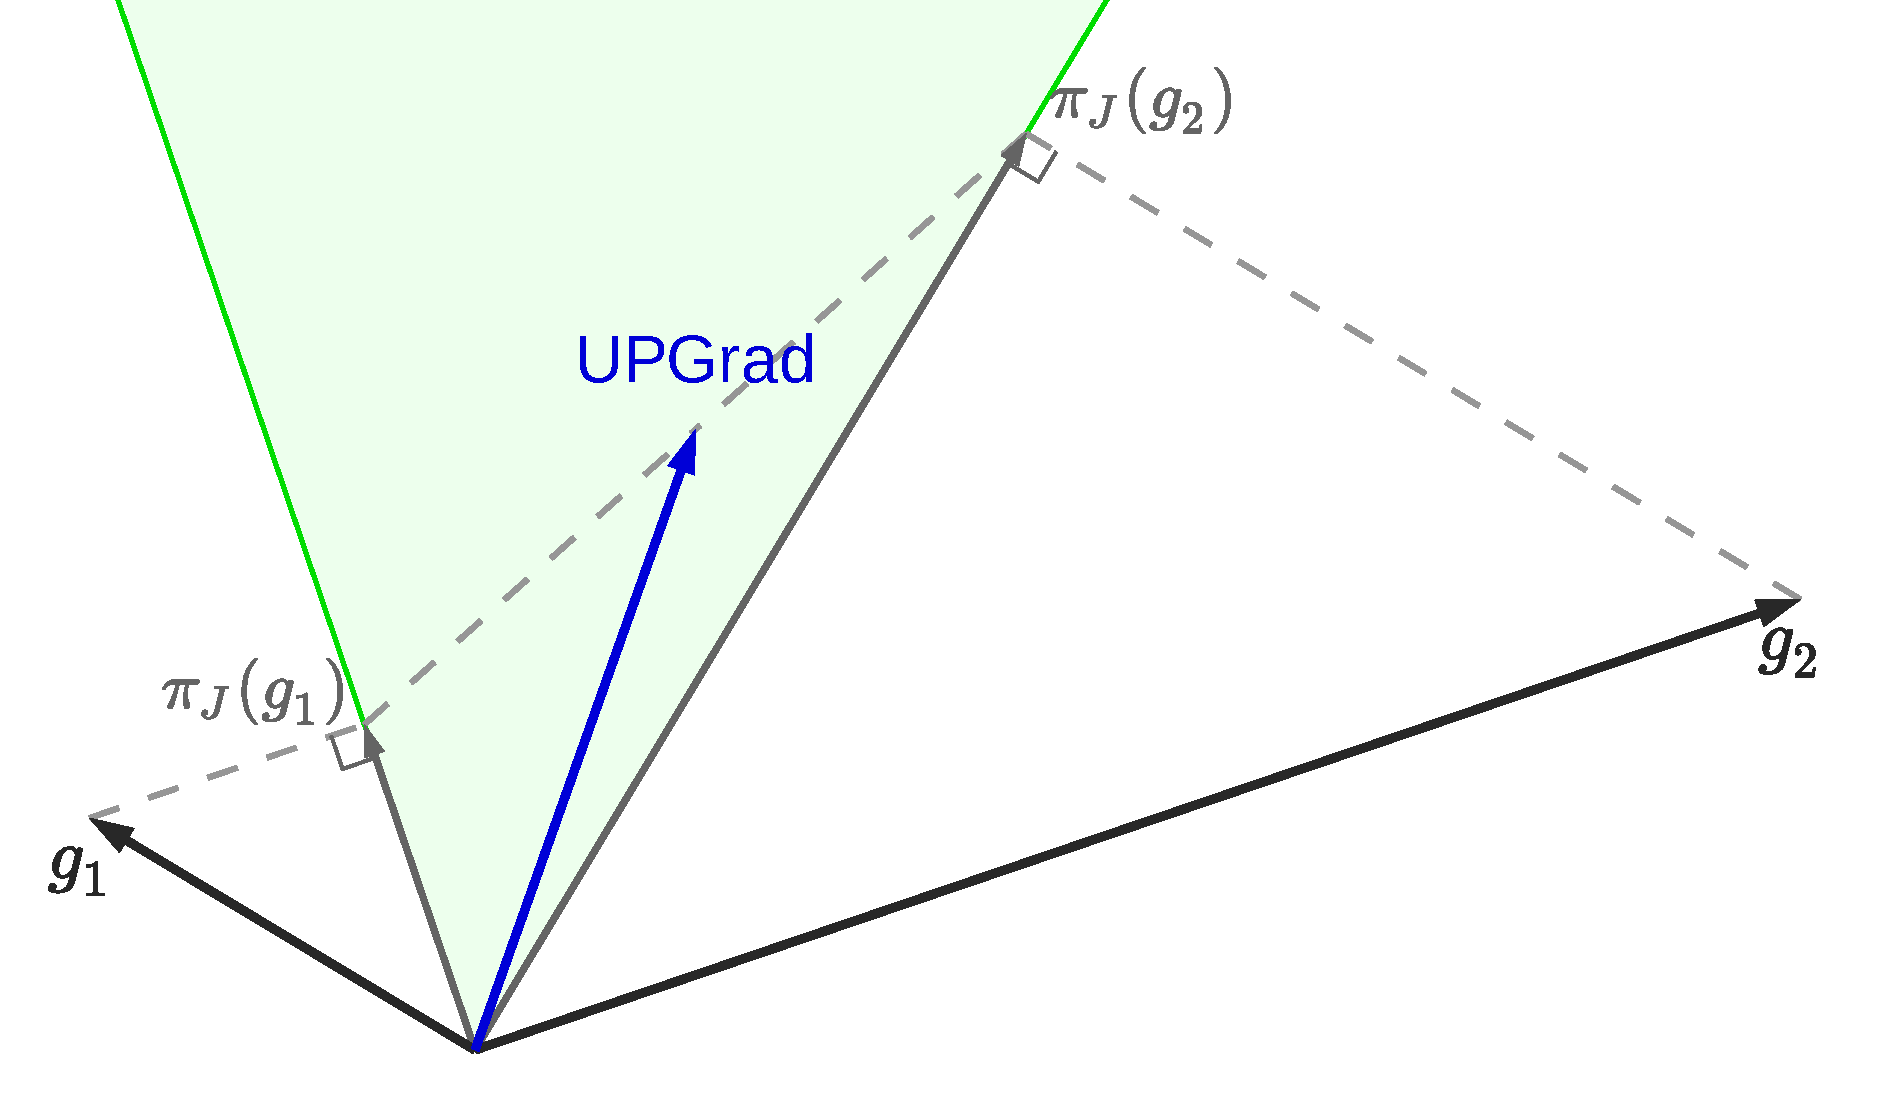
\includegraphics[width=0.95\linewidth]{images/direction_upgrad.pdf}\\[2mm]
        {\small (a) $\upgrad$ never conflicts with $\vg_1$ or $\vg_2$.\par}
        \vspace{6mm}
        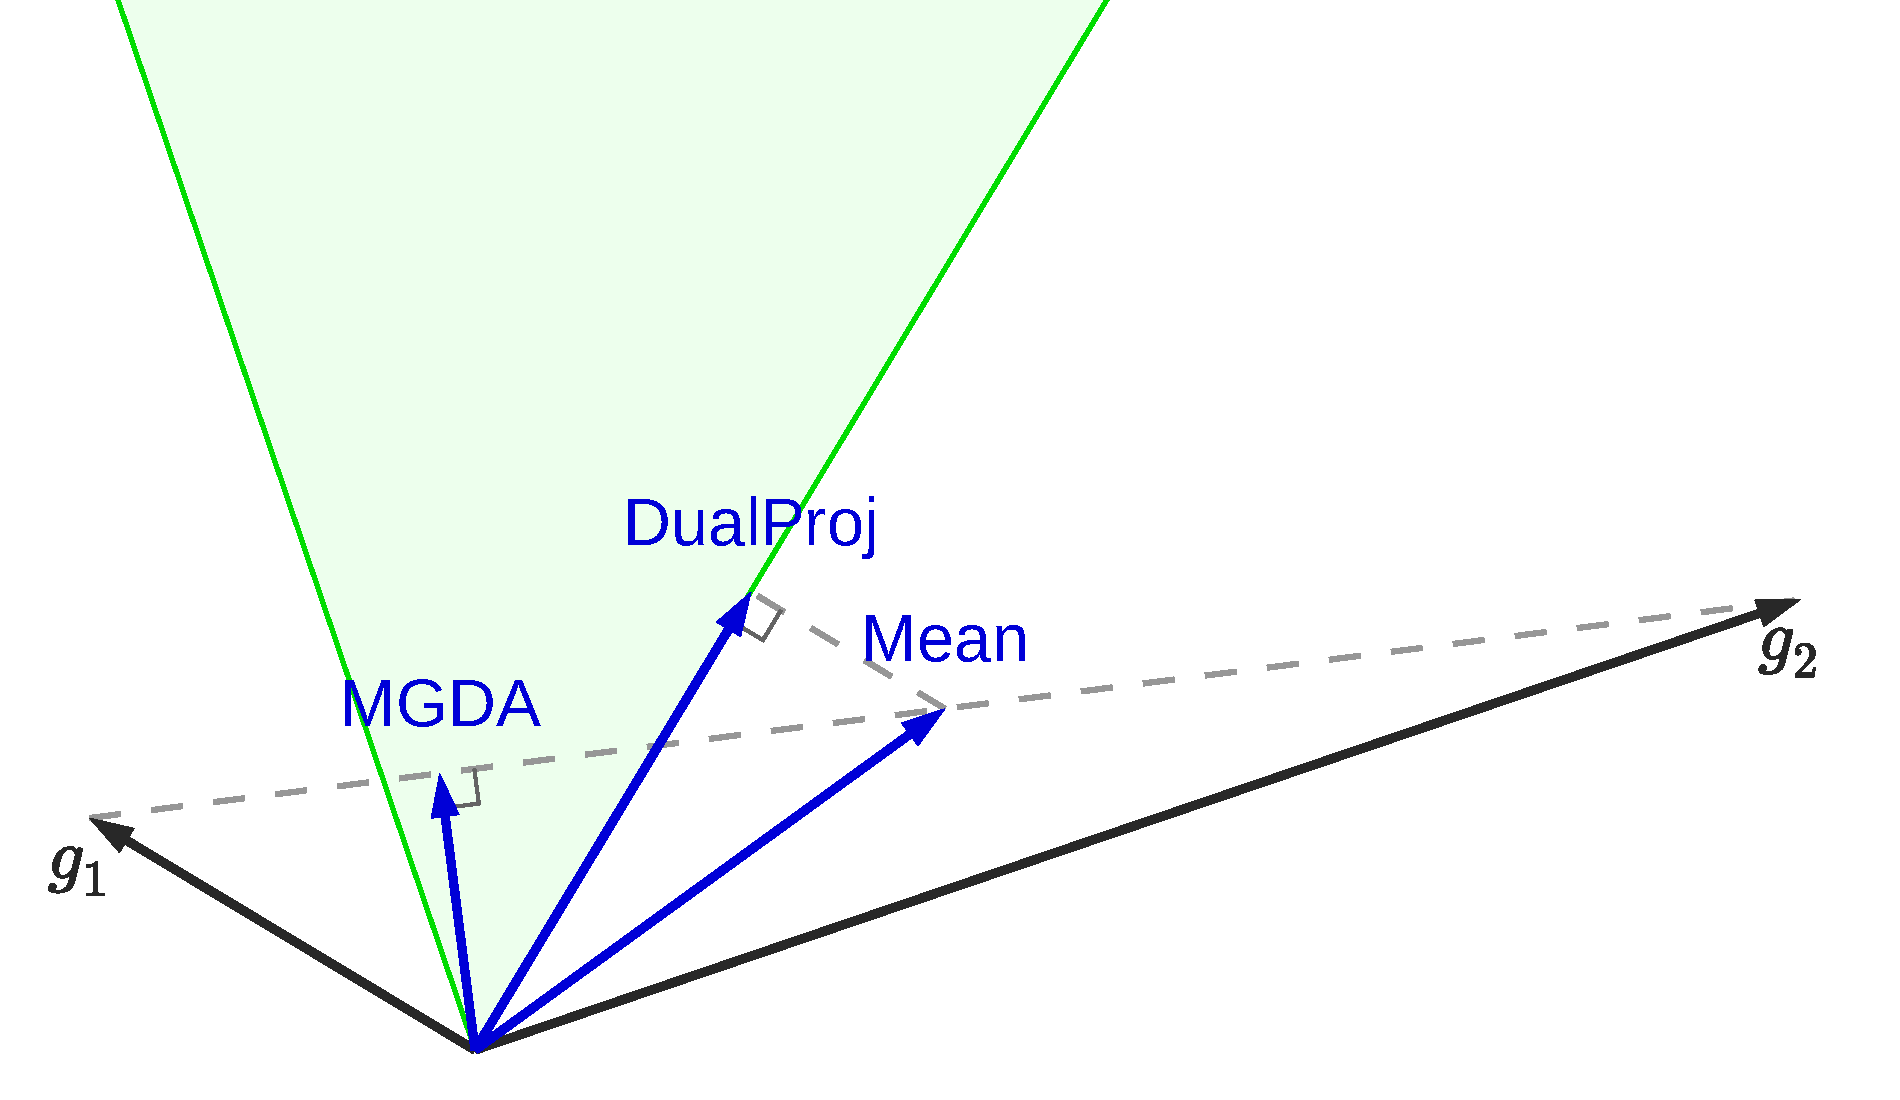
\includegraphics[width=0.95\linewidth]{images/directions.pdf}\\[2mm]
        {\small (b) $\meanagg$ conflicts with $\vg_1$. $\dualproj$ lands on the cone's boundary.
        $\mgda$ is almost orthogonal to $\vg_2$ because of its larger norm.\par}
    \end{center}
    \vspace{-5mm}
    \[
        \upgrad(\J)=\frac{1}{m}\sum_{i=1}^m \proj_\J(\vg_i),
        \qquad
        \proj_\J(\vx)= \argmin_{\vy:\;\0\pleq \J \vy} \| \vy-\vx \|^2
    \]
    \begin{itemize}
        \item Satisfies \hl{all three properties}.
        \item If no two gradients conflict, it is simply the \textbf{mean}.
    \end{itemize}
}

\posterbox[adjusted title=Convergence to the Pareto front]{name=convergence, column=3, below=takeaway}{
    \begin{keybox}
        \textbf{Theorem.}
        Let $\vf$ be $\beta$-smooth and $\pleq$-convex, with a compact Pareto front.
        JD with $\upgrad$ and step size $\eta=\frac{1}{\beta\sqrt m}$ (with bounded weights) makes $\vf(\vx_t)$
        \textbf{converge to the Pareto front}.
    \end{keybox}
    Usual guarantees only reach a \emph{weakly Pareto stationary} point, which can be far from optimal even for convex $\vf$.
    $\upgrad$ is the \textbf{first non-conflicting aggregator} proven to reach the Pareto front in this setting.

    \begin{center}
        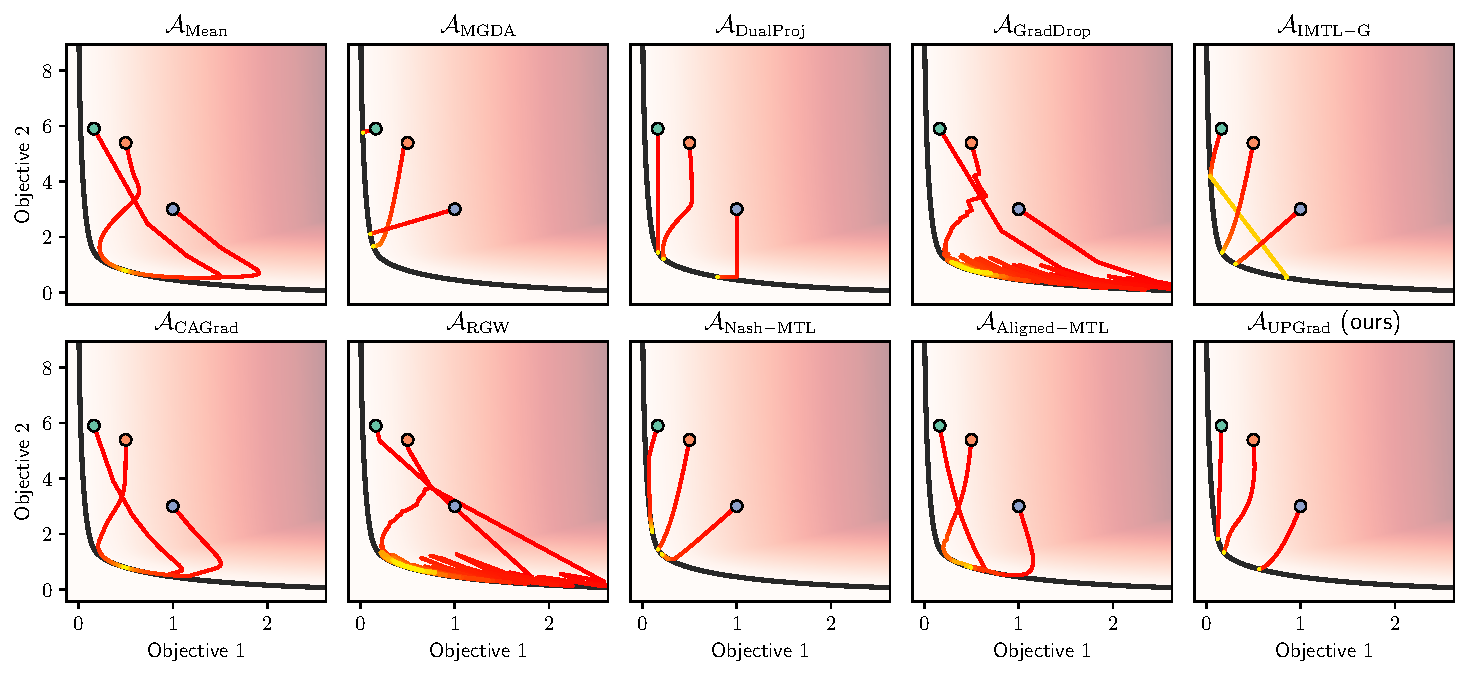
\includegraphics[width=\linewidth]{images/CQF_values.pdf}
    \end{center}
    \vspace{-4mm}
    {\small Trajectories in objective space on a convex quadratic $\vf:\R^2\to\R^2$ (black: Pareto front).\par}
}

%%%%%%%%%%%%%%%%%%%%%%%%%%%%%%%%%%%%%%%%%%%%%%%%%%%%%%%%%%%%%%%%%%%%%%%%%%%%%%%%%%%%%%%%%%%%%%%%%%%%%%%%%%%%%%%%%%%%%%%%%%
% Column 3
\posterbox[adjusted title=Instance-wise risk minimization]{name=iwrm, column=4, below=takeaway}{
    Treat the \textbf{loss of each training example as its own objective}:
    \[
        \underbrace{\bar f(\vtheta)=\frac1m\sum_{i=1}^m f_i(\vtheta)}_{\text{ERM}}
        \qquad\longrightarrow\qquad
        \underbrace{\vf(\vtheta)=\begin{bmatrix}f_1(\vtheta)&\cdots&f_m(\vtheta)\end{bmatrix}^\T}_{\text{IWRM (ours)}}
    \]
    Optimized with SSJD on mini-batches. With $\meanagg$, this is exactly SGD.
    \vspace{-6mm}

    \begin{center}
        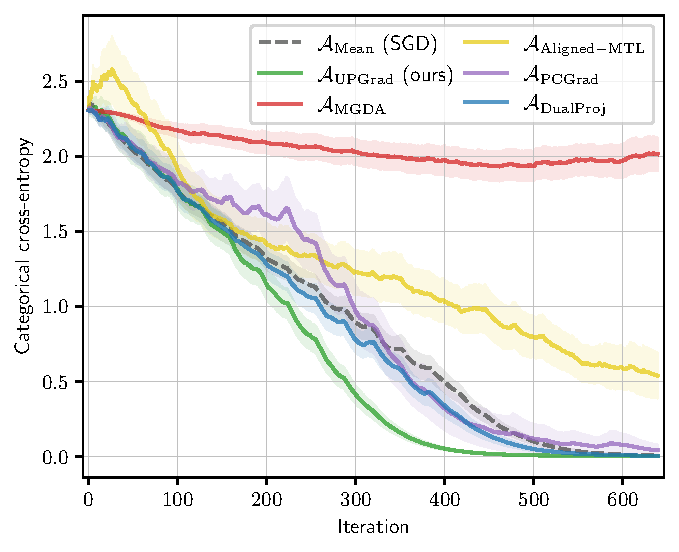
\includegraphics[width=0.7\linewidth]{images/cifar10_train_losses.pdf}
    \end{center}
    \vspace{-4mm}
    {\small CIFAR-10 (1024 images, batch size 32): $\upgrad$ \textbf{minimizes the average training loss faster than SGD}, the method that directly targets it.\par}

    \begin{center}
        \small
        \rowcolors{2}{tablerow}{}
        \begin{tabular}{lcccccc}
            \toprule
            Test acc. (\%) & SVHN & CIFAR-10 & EuroSAT & MNIST & F-MNIST & K-MNIST \\
            \midrule
            $\meanagg$ (SGD) & 69.6 & 47.7 & 68.5 & \textbf{96.3} & 80.7 & 76.9 \\
            $\upgrad$ & \textbf{69.7} & \textbf{48.1} & \textbf{73.0} & 96.0 & 80.8 & \textbf{77.1} \\
            $\dualproj$ & 69.3 & 47.2 & 72.7 & 96.1 & 80.8 & 76.4 \\
            $\graddrop$ & 68.9 & 46.8 & 71.9 & \textbf{96.3} & \textbf{80.9} & 76.9 \\
            $\mgda$ & 41.7 & 32.9 & 62.5 & 85.2 & 73.4 & 53.7 \\
            \bottomrule
        \end{tabular}
    \end{center}
}

\posterbox[adjusted title=Gramian-based Jacobian descent]{name=gramian, column=3, between=convergence and bottom}{
    For weighted aggregators with weights $\W(\G)$ depending only on the Gramian $\G=\J\J^\T$:
    \[
        \A\big(\jac \vf(\vx)\big) = \nabla \Big(\W\big(\gram \vf(\vx)\big)^\T \vf\Big)(\vx)
    \]
    For $\upgrad$, by duality, $\proj_\J(\J^\T\vu)=\J^\T\vw$ where $\vw$ solves an $m$-dimensional QP that only depends on the Gramian:
    \[
        \vw\in\argmin_{\vv:\;\vu\pleq \vv}\; \vv^\T \G \vv
    \]
    A step needs only the \textbf{$m\times m$ Gramian} and \textbf{one backward pass}.
    Like gradients, Gramians can be backpropagated, \textbf{without ever storing the Jacobian}:
    \begin{align*}
        \text{(chain rule)}\quad & \gram (\vf\circ \vg)(\vx)=\jac \vf\big(\vg(\vx)\big)\; \gram \vg(\vx)\; \jac \vf\big(\vg(\vx)\big)^\T\\[2mm]
        \text{(sum rule)}\quad & \gram \vf(\vx_1, \dots, \vx_k)=\sum_{i=1}^k \gram_{\vx_i} \vf(\vx_1,\dots, \vx_k)
    \end{align*}

    \begin{center}
        \Large Memory: $\bigo(mn)\;\to\;\bigo(n+m^2)$\\[3mm]
        \large \hl{87--93\% less memory}\qquad\hl{42--89\% faster}
    \end{center}
}

\posterbox[adjusted title=TorchJD: JD in PyTorch]{name=torchjd, column=4, between=iwrm and bottom}{
    \begin{keybox}[halign=center]
        \Large\ttfamily\bfseries pip install "torchjd[quadprog\_projector]"
    \end{keybox}
\lstinputlisting[style=pythonstyle]{code/usage.py}
    \begin{center}
        \href{https://github.com/SimplexLab/TorchJD}{github.com/SimplexLab/TorchJD}
    \end{center}
}

\end{tcbposter}
\end{document}
